\documentclass[a4paper,twocolumn]{article}  % If you prefer single cloumn setup, just remove the "twocolumn" option
\usepackage{fontspec}   %加這個就可以設定字體
\usepackage{xeCJK}       %讓中英文字體分開設置
\usepackage{indentfirst}
\usepackage{listings}
\usepackage[newfloat]{minted}
\usepackage{float}
\usepackage{graphicx}
\usepackage{caption}
\usepackage{fancyhdr}
\usepackage{hyperref}
\usepackage{amsmath}
\usepackage{multirow}
\usepackage[dvipsnames]{xcolor}
\usepackage{graphicx}
\usepackage{tabularx}
\usepackage{booktabs}
\usepackage{caption}
\usepackage{subcaption}
\usepackage{pifont}
\usepackage{amssymb}
\usepackage[backend=biber]{biblatex}
\addbibresource{template.bib}


\usepackage{pdftexcmds}
\usepackage{catchfile}
\usepackage{ifluatex}
\usepackage{ifplatform}

\usepackage[breakable, listings, skins, minted]{tcolorbox}
\usepackage{etoolbox}
\setminted{fontsize=\footnotesize}
\renewtcblisting{minted}{%
    listing engine=minted,
    minted language=python,
    listing only,
    breakable,
    enhanced,
    minted options = {
        linenos, 
        breaklines=true, 
        breakbefore=., 
        % fontsize=\footnotesize, 
        numbersep=2mm
    },
    overlay={%
        \begin{tcbclipinterior}
            \fill[gray!25] (frame.south west) rectangle ([xshift=4mm]frame.north west);
        \end{tcbclipinterior}
    }   
}

\usepackage[
top=1.5cm,
bottom=0.75cm,
left=1.25cm,
right=1.25cm,
includehead,includefoot,
heightrounded, % to avoid spurious underfull messages
]{geometry} 

\newenvironment{code}{\captionsetup{type=listing}}{}
\SetupFloatingEnvironment{listing}{name=Code}

\title{A Report Template for CS Students}
\author{Jie-Ying Lee 李杰穎}
\date{\today}


\setCJKmainfont{Noto Serif TC}  % 設定你想要的中文字體

\ifwindows
\setmonofont[Mapping=tex-text]{Consolas}
\fi

\XeTeXlinebreaklocale "zh"             %這兩行一定要加,中文才能自動換行
\XeTeXlinebreakskip = 0pt plus 1pt     %這兩行一定要加,中文才能自動換行

\newcommand*{\dif}{\mathop{}\!\mathrm{d}}

\begin{document}
\maketitle
\section{Introduction}

This report template aims to help CS students creating beautiful report using \LaTeX. It natively supports Chinese character, code highlighting and reference using the biber backend\footnote{You can insert footnote like this. This report template follow MIT License, please refer to LICENSE for more detail.}.

\section{A section}
\subsection{A subsection}
\subsubsection{A subsubsection}

The U-Net architecture forms the backbone of the diffusion model. My implementation follows the standard U-Net structure with skip connections, but is enhanced with conditioning mechanisms throughout the network:


% A code block demo, support code highlighting
\begin{code}
\captionof{listing}{\textbf{Implementation of the conditional U-Net architecture}}
\begin{minted}
class ConditionalUNet(nn.Module):
    def __init__(self, in_channels=3, model_channels=64, out_channels=3, num_classes=24, 
                 time_dim=256, use_adagn=False, num_groups=8, device="cuda"):
        super().__init__()
        # Embedding dimensions and layers
        self.emb_dim = time_dim * 2  # Combined embedding dimension
        
        # Time and label embedding networks
        self.time_mlp = nn.Sequential(
            SinusoidalPositionEmbeddings(time_dim),
            nn.Linear(time_dim, time_dim),
            nn.SiLU(),
            nn.Linear(time_dim, time_dim)
        )
        
        self.label_emb = nn.Sequential(
            nn.Linear(num_classes, time_dim),
            nn.SiLU(),
            nn.Linear(time_dim, time_dim)
        )
        
        # Encoder (downsampling) path
        self.conv_in = nn.Conv2d(in_channels, model_channels, kernel_size=3, padding=1)
        self.down1 = Block(model_channels, model_channels*2, self.emb_dim, up=False, use_adagn=use_adagn)
        self.down2 = Block(model_channels*2, model_channels*4, self.emb_dim, up=False, use_adagn=use_adagn)
        self.down3 = Block(model_channels*4, model_channels*8, self.emb_dim, up=False, use_adagn=use_adagn)
        
        # Bottleneck
        self.bottleneck1 = nn.Conv2d(model_channels*8, model_channels*8, kernel_size=3, padding=1)
        self.bottleneck2 = nn.Conv2d(model_channels*8, model_channels*8, kernel_size=3, padding=1)
        
        # Decoder (upsampling) path with skip connections
        self.up1 = Block(model_channels*8, model_channels*4, self.emb_dim, up=True, use_adagn=use_adagn)
        self.up2 = Block(model_channels*4, model_channels*2, self.emb_dim, up=True, use_adagn=use_adagn)
        self.up3 = Block(model_channels*2, model_channels, self.emb_dim, up=True, use_adagn=use_adagn)
        
        # Output projection
        self.conv_out = nn.Sequential(
            nn.Conv2d(model_channels, model_channels, kernel_size=3, padding=1),
            nn.GroupNorm(num_groups, model_channels) if use_adagn else nn.BatchNorm2d(model_channels),
            nn.SiLU(),
            nn.Conv2d(model_channels, out_channels, kernel_size=3, padding=1)
        )

    def forward(self, x, t, labels):
        # Embed time and labels
        t_emb = self.time_mlp(t)
        c_emb = self.label_emb(labels)
        
        # Concatenate time and label embeddings instead of adding
        emb = torch.cat([t_emb, c_emb], dim=1)
        
        # Initial conv
        x = self.conv_in(x)
        
        # Downsample
        d1 = self.down1(x, emb)
        d2 = self.down2(d1, emb)
        d3 = self.down3(d2, emb)
        
        # Bottleneck
        bottleneck = self.bottleneck1(d3)
        
        # Apply normalization to bottleneck
        if self.use_adagn:
            # Use AdaGroupNorm from diffusers
            bottleneck = self.bottleneck_norm1(bottleneck, emb)
            bottleneck = F.silu(bottleneck)
        else:
            bottleneck = self.bottleneck_norm1(bottleneck)
            bottleneck = F.silu(bottleneck)
            
        bottleneck = self.bottleneck2(bottleneck)
        
        # Apply normalization to bottleneck
        if self.use_adagn:
            # Use AdaGroupNorm from diffusers
            bottleneck = self.bottleneck_norm2(bottleneck, emb)
            bottleneck = F.silu(bottleneck)
        else:
            bottleneck = self.bottleneck_norm2(bottleneck)
            bottleneck = F.silu(bottleneck)
        
        # Upsample with skip connections
        up1 = self.up1(torch.cat([bottleneck, d3], dim=1), emb)
        up2 = self.up2(torch.cat([up1, d2], dim=1), emb)
        up3 = self.up3(torch.cat([up2, d1], dim=1), emb)
        
        # Output
        return self.conv_out(up3)
\end{minted}
\end{code}

The network progressively reduces the spatial dimensions while increasing the channel count in the encoder path, and then reverses this process in the decoder path, using skip connections to preserve spatial information. The conditioning information is incorporated at each block, allowing it to influence the denoising process at multiple levels of abstraction.

\subsection{DDPM}

The Denoising Diffusion Probabilistic Model (DDPM)~\cite{ho2020denoising} framework forms the core of my image generation system. The DDPM class implements both the forward noising process and the reverse denoising process for sampling:

\begin{code}
\captionof{listing}{\textbf{Implementation of the DDPM class}}
\begin{minted}
class DDPM(nn.Module):
    def __init__(self, model, beta_start=1e-4, beta_end=0.02, timesteps=1000, 
                 beta_schedule="linear", device="cuda"):
        super().__init__()
        self.model = model
        self.timesteps = timesteps
        self.device = device
        
        # Define beta schedule
        if beta_schedule == "linear":
            self.betas = torch.linspace(beta_start, beta_end, timesteps, device=device)
        elif beta_schedule == "cosine":
            self.betas = cosine_beta_schedule(timesteps, device=device)
        
        # Pre-calculate diffusion parameters
        self.alphas = 1. - self.betas
        self.alphas_cumprod = torch.cumprod(self.alphas, axis=0)
        self.alphas_cumprod_prev = F.pad(self.alphas_cumprod[:-1], (1, 0), value=1.0)
        
        # Calculations for diffusion q(x_t | x_{t-1}) and others
        self.sqrt_alphas_cumprod = torch.sqrt(self.alphas_cumprod)
        self.sqrt_one_minus_alphas_cumprod = torch.sqrt(1. - self.alphas_cumprod)
        self.log_one_minus_alphas_cumprod = torch.log(1. - self.alphas_cumprod)
        self.sqrt_recip_alphas_cumprod = torch.sqrt(1. / self.alphas_cumprod)
        self.sqrt_recipm1_alphas_cumprod = torch.sqrt(1. / self.alphas_cumprod - 1)
\end{minted}
\end{code}


\paragraph{Denoising process.} In \autoref{fig:denoisingprocess}, I visualize the denoising process at timestep 0, 100, 200, 300, 400, 500, 600, 700, 800, 900 and 999.

\begin{figure}[H]
\centering
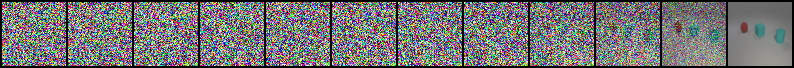
\includegraphics[width=0.95\linewidth]{figures/denoising_process}
\caption{The denoising process of synthesizing image contain, ``red sphere'', ``cyan
cylinder'' and ``cyan cube''. Use cosine $\beta$ scheduling}
\label{fig:denoisingprocess}
\end{figure}


\printbibliography
\end{document}